%\documentclass[preview]{standalone}
\documentclass{standalone}

\usepackage{fontspec}
\setmainfont[Ligatures=TeX, Mapping=tex-text]{Lato}
\usepackage{tikz}
\usetikzlibrary{arrows.meta}
\usepackage{xfp}

\begin{document}
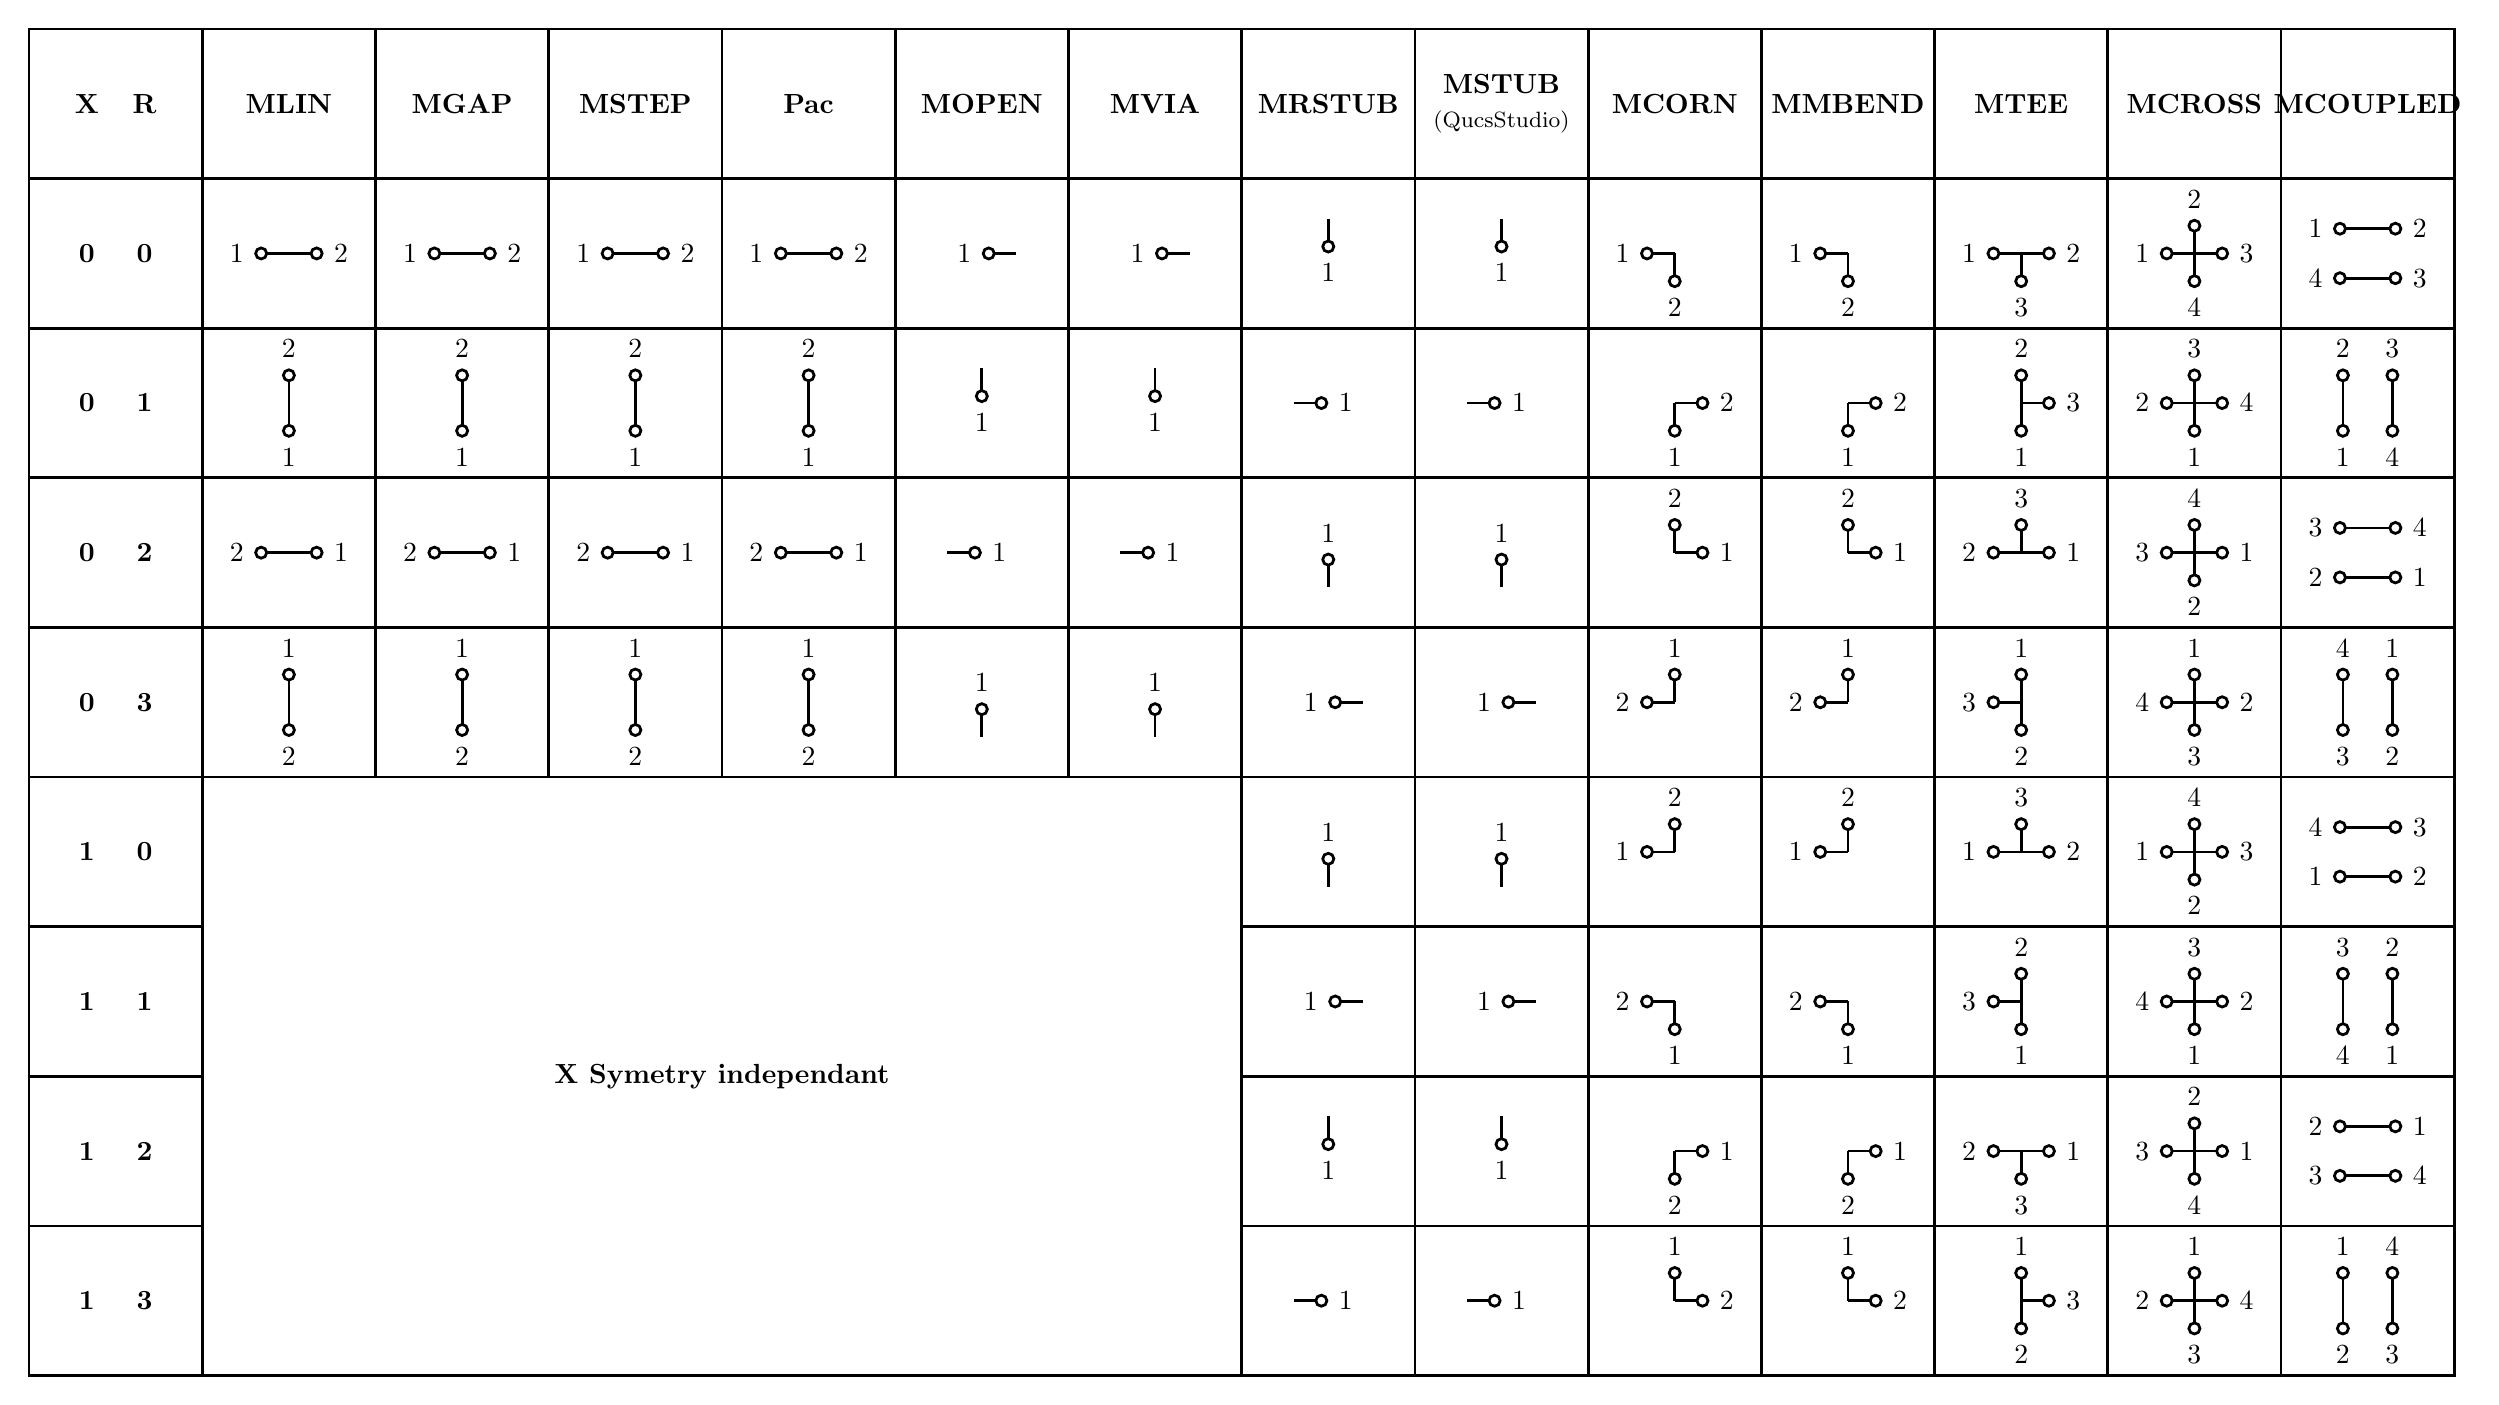
\begin{tikzpicture}

\def\stepx{2.2}
\def\stepy{1.9}
\def\rows{9}
\def\cols{14}

% GRID
\draw [line width=1pt, join=miter] (0,0)
	rectangle (\fpeval{\cols*\stepx},\fpeval{\rows*\stepy});
\draw [line width=1pt] (0,0) grid[xstep=\stepx, ystep=\stepy]
	(\fpeval{\cols*\stepx},\fpeval{\rows*\stepy});
\filldraw [line width=1pt, fill=white] (\fpeval{1*\stepx},0)
	rectangle +(\fpeval{6*\stepx},\fpeval{4*\stepy})
	+(\fpeval{6*\stepx/2},\fpeval{4*\stepy/2}) node {\textbf{X Symetry independant}};

% XR
\draw (\fpeval{1*\stepx-\stepx/2-\stepx/6},\fpeval{9*\stepy-\stepy/2}) node(x) {\textbf{X}}
	+(0,\fpeval{-1*\stepy}) node {\textbf{0}}
	+(0,\fpeval{-2*\stepy}) node {\textbf{0}}
	+(0,\fpeval{-3*\stepy}) node {\textbf{0}}
	+(0,\fpeval{-4*\stepy}) node {\textbf{0}}
	+(0,\fpeval{-5*\stepy}) node {\textbf{1}}
	+(0,\fpeval{-6*\stepy}) node {\textbf{1}}
	+(0,\fpeval{-7*\stepy}) node {\textbf{1}}
	+(0,\fpeval{-8*\stepy}) node {\textbf{1}};
\draw (\fpeval{1*\stepx-\stepx/2+\stepx/6},\fpeval{9*\stepy-\stepy/2}) node(r) {\textbf{R}}
	+(0,\fpeval{-1*\stepy}) node {\textbf{0}}
	+(0,\fpeval{-2*\stepy}) node {\textbf{1}}
	+(0,\fpeval{-3*\stepy}) node {\textbf{2}}
	+(0,\fpeval{-4*\stepy}) node {\textbf{3}}
	+(0,\fpeval{-5*\stepy}) node {\textbf{0}}
	+(0,\fpeval{-6*\stepy}) node {\textbf{1}}
	+(0,\fpeval{-7*\stepy}) node {\textbf{2}}
	+(0,\fpeval{-8*\stepy}) node {\textbf{3}};

% MLIN
\draw (\fpeval{2*\stepx-\stepx/2},\fpeval{9*\stepy-\stepy/2}) node(mlin) {\textbf{MLIN}};
	\draw [line width=1pt, -{Circle[open, length=5pt]}] (mlin) ++(0,\fpeval{-1*\stepy})
		-- +(\fpeval{\stepx/-5},0) node[left] {1};
	\draw [line width=1pt, -{Circle[open, length=5pt]}] (mlin) ++(0,\fpeval{-1*\stepy})
		-- +(\fpeval{\stepx/5},0) node[right] {2};

	\draw [line width=1pt, -{Circle[open, length=5pt]}] (mlin) ++(0,\fpeval{-2*\stepy})
		-- +(0,\fpeval{\stepx/-5}) node[below] {1};
	\draw [line width=1pt, -{Circle[open, length=5pt]}] (mlin) ++(0,\fpeval{-2*\stepy})
		-- +(0,\fpeval{\stepx/5}) node[above] {2};

	\draw [line width=1pt, -{Circle[open, length=5pt]}] (mlin) ++(0,\fpeval{-3*\stepy})
		-- +(\fpeval{\stepx/5},0) node[right] {1};
	\draw [line width=1pt, -{Circle[open, length=5pt]}] (mlin) ++(0,\fpeval{-3*\stepy})
		-- +(\fpeval{\stepx/-5},0) node[left] {2};

	\draw [line width=1pt, -{Circle[open, length=5pt]}] (mlin) ++(0,\fpeval{-4*\stepy})
		-- +(0,\fpeval{\stepx/5}) node[above] {1};
	\draw [line width=1pt, -{Circle[open, length=5pt]}] (mlin) ++(0,\fpeval{-4*\stepy})
		-- +(0,\fpeval{\stepx/-5}) node[below] {2};

% MGAP
\draw (\fpeval{3*\stepx-\stepx/2},\fpeval{9*\stepy-\stepy/2}) node(mgap) {\textbf{MGAP}};
	\draw [line width=1pt, -{Circle[open, length=5pt]}] (mgap) ++(0,\fpeval{-1*\stepy})
		-- +(\fpeval{\stepx/-5},0) node[left] {1};
	\draw [line width=1pt, -{Circle[open, length=5pt]}] (mgap) ++(0,\fpeval{-1*\stepy})
		-- +(\fpeval{\stepx/5},0) node[right] {2};

	\draw [line width=1pt, -{Circle[open, length=5pt]}] (mgap) ++(0,\fpeval{-2*\stepy})
		-- +(0,\fpeval{\stepx/-5}) node[below] {1};
	\draw [line width=1pt, -{Circle[open, length=5pt]}] (mgap) ++(0,\fpeval{-2*\stepy})
		-- +(0,\fpeval{\stepx/5}) node[above] {2};

	\draw [line width=1pt, -{Circle[open, length=5pt]}] (mgap) ++(0,\fpeval{-3*\stepy})
		-- +(\fpeval{\stepx/5},0) node[right] {1};
	\draw [line width=1pt, -{Circle[open, length=5pt]}] (mgap) ++(0,\fpeval{-3*\stepy})
		-- +(\fpeval{\stepx/-5},0) node[left] {2};

	\draw [line width=1pt, -{Circle[open, length=5pt]}] (mgap) ++(0,\fpeval{-4*\stepy})
		-- +(0,\fpeval{\stepx/5}) node[above] {1};
	\draw [line width=1pt, -{Circle[open, length=5pt]}] (mgap) ++(0,\fpeval{-4*\stepy})
		-- +(0,\fpeval{\stepx/-5}) node[below] {2};

% MSTEP
\draw (\fpeval{4*\stepx-\stepx/2},\fpeval{9*\stepy-\stepy/2}) node(mstep) {\textbf{MSTEP}};
	\draw [line width=1pt, -{Circle[open, length=5pt]}] (mstep) ++(0,\fpeval{-1*\stepy})
		-- +(\fpeval{\stepx/-5},0) node[left] {1};
	\draw [line width=1pt, -{Circle[open, length=5pt]}] (mstep) ++(0,\fpeval{-1*\stepy})
		-- +(\fpeval{\stepx/5},0) node[right] {2};

	\draw [line width=1pt, -{Circle[open, length=5pt]}] (mstep) ++(0,\fpeval{-2*\stepy})
		-- +(0,\fpeval{\stepx/-5}) node[below] {1};
	\draw [line width=1pt, -{Circle[open, length=5pt]}] (mstep) ++(0,\fpeval{-2*\stepy})
		-- +(0,\fpeval{\stepx/5}) node[above] {2};

	\draw [line width=1pt, -{Circle[open, length=5pt]}] (mstep) ++(0,\fpeval{-3*\stepy})
		-- +(\fpeval{\stepx/5},0) node[right] {1};
	\draw [line width=1pt, -{Circle[open, length=5pt]}] (mstep) ++(0,\fpeval{-3*\stepy})
		-- +(\fpeval{\stepx/-5},0) node[left] {2};

	\draw [line width=1pt, -{Circle[open, length=5pt]}] (mstep) ++(0,\fpeval{-4*\stepy})
		-- +(0,\fpeval{\stepx/5}) node[above] {1};
	\draw [line width=1pt, -{Circle[open, length=5pt]}] (mstep) ++(0,\fpeval{-4*\stepy})
		-- +(0,\fpeval{\stepx/-5}) node[below] {2};

% PAC
\draw (\fpeval{5*\stepx-\stepx/2},\fpeval{9*\stepy-\stepy/2}) node(pac) {\textbf{Pac}};
	\draw [line width=1pt, -{Circle[open, length=5pt]}] (pac) ++(0,\fpeval{-1*\stepy})
		-- +(\fpeval{\stepx/-5},0) node[left] {1};
	\draw [line width=1pt, -{Circle[open, length=5pt]}] (pac) ++(0,\fpeval{-1*\stepy})
		-- +(\fpeval{\stepx/5},0) node[right] {2};

	\draw [line width=1pt, -{Circle[open, length=5pt]}] (pac) ++(0,\fpeval{-2*\stepy})
		-- +(0,\fpeval{\stepx/-5}) node[below] {1};
	\draw [line width=1pt, -{Circle[open, length=5pt]}] (pac) ++(0,\fpeval{-2*\stepy})
		-- +(0,\fpeval{\stepx/5}) node[above] {2};

	\draw [line width=1pt, -{Circle[open, length=5pt]}] (pac) ++(0,\fpeval{-3*\stepy})
		-- +(\fpeval{\stepx/5},0) node[right] {1};
	\draw [line width=1pt, -{Circle[open, length=5pt]}] (pac) ++(0,\fpeval{-3*\stepy})
		-- +(\fpeval{\stepx/-5},0) node[left] {2};

	\draw [line width=1pt, -{Circle[open, length=5pt]}] (pac) ++(0,\fpeval{-4*\stepy})
		-- +(0,\fpeval{\stepx/5}) node[above] {1};
	\draw [line width=1pt, -{Circle[open, length=5pt]}] (pac) ++(0,\fpeval{-4*\stepy})
		-- +(0,\fpeval{\stepx/-5}) node[below] {2};

% MOPEN
\draw (\fpeval{6*\stepx-\stepx/2},\fpeval{9*\stepy-\stepy/2}) node(mopen) {\textbf{MOPEN}};
	\draw [line width=1pt, -{Circle[open, length=5pt]}] (mopen) ++(0,\fpeval{-1*\stepy})
		++(\fpeval{\stepx/5},0) -- +(\fpeval{\stepx/-5},0) node[left] {1};

	\draw [line width=1pt, -{Circle[open, length=5pt]}] (mopen) ++(0,\fpeval{-2*\stepy})
		++(0,\fpeval{\stepx/5}) -- +(0,\fpeval{\stepx/-5}) node[below] {1};

	\draw [line width=1pt, -{Circle[open, length=5pt]}] (mopen) ++(0,\fpeval{-3*\stepy})
		++(\fpeval{\stepx/-5},0) -- +(\fpeval{\stepx/5},0) node[right] {1};

	\draw [line width=1pt, -{Circle[open, length=5pt]}] (mopen) ++(0,\fpeval{-4*\stepy})
		++(0,\fpeval{\stepx/-5}) -- +(0,\fpeval{\stepx/5}) node[above] {1};

% MVIA
\draw (\fpeval{7*\stepx-\stepx/2},\fpeval{9*\stepy-\stepy/2}) node(mvia) {\textbf{MVIA}};
	\draw [line width=1pt, -{Circle[open, length=5pt]}] (mvia) ++(0,\fpeval{-1*\stepy})
		++(\fpeval{\stepx/5},0) -- +(\fpeval{\stepx/-5},0) node[left] {1};

	\draw [line width=1pt, -{Circle[open, length=5pt]}] (mvia) ++(0,\fpeval{-2*\stepy})
		++(0,\fpeval{\stepx/5}) -- +(0,\fpeval{\stepx/-5}) node[below] {1};

	\draw [line width=1pt, -{Circle[open, length=5pt]}] (mvia) ++(0,\fpeval{-3*\stepy})
		++(\fpeval{\stepx/-5},0) -- +(\fpeval{\stepx/5},0) node[right] {1};

	\draw [line width=1pt, -{Circle[open, length=5pt]}] (mvia) ++(0,\fpeval{-4*\stepy})
		++(0,\fpeval{\stepx/-5}) -- +(0,\fpeval{\stepx/5}) node[above] {1};

% MRSTUB
\draw (\fpeval{8*\stepx-\stepx/2},\fpeval{9*\stepy-\stepy/2}) node(mrstub) {\textbf{MRSTUB}};
	\draw [line width=1pt, -{Circle[open, length=5pt]}] (mrstub) ++(0,\fpeval{-1*\stepy})
		++(0,\fpeval{\stepx/5}) -- +(0,\fpeval{\stepx/-5}) node[below] {1};

	\draw [line width=1pt, -{Circle[open, length=5pt]}] (mrstub) ++(0,\fpeval{-2*\stepy})
		++(\fpeval{\stepx/-5},0) -- +(\fpeval{\stepx/5},0) node[right] {1};

	\draw [line width=1pt, -{Circle[open, length=5pt]}] (mrstub) ++(0,\fpeval{-3*\stepy})
		++(0,\fpeval{\stepx/-5}) -- +(0,\fpeval{\stepx/5}) node[above] {1};

	\draw [line width=1pt, -{Circle[open, length=5pt]}] (mrstub) ++(0,\fpeval{-4*\stepy})
		++(\fpeval{\stepx/5},0) -- +(\fpeval{\stepx/-5},0) node[left] {1};

	\draw [line width=1pt, -{Circle[open, length=5pt]}] (mrstub) ++(0,\fpeval{-5*\stepy})
		++(0,\fpeval{\stepx/-5}) -- +(0,\fpeval{\stepx/5}) node[above] {1};

	\draw [line width=1pt, -{Circle[open, length=5pt]}] (mrstub) ++(0,\fpeval{-6*\stepy})
		++(\fpeval{\stepx/5},0) -- +(\fpeval{\stepx/-5},0) node[left] {1};

	\draw [line width=1pt, -{Circle[open, length=5pt]}] (mrstub) ++(0,\fpeval{-7*\stepy})
		++(0,\fpeval{\stepx/5}) -- +(0,\fpeval{\stepx/-5}) node[below] {1};

	\draw [line width=1pt, -{Circle[open, length=5pt]}] (mrstub) ++(0,\fpeval{-8*\stepy})
		++(\fpeval{\stepx/-5},0) -- +(\fpeval{\stepx/5},0) node[right] {1};

% MSTUB
\draw (\fpeval{9*\stepx-\stepx/2},\fpeval{9*\stepy-\stepy/2}) node[align=center](mstub) {\textbf{MSTUB}\\\footnotesize(QucsStudio)};
	\draw [line width=1pt, -{Circle[open, length=5pt]}] (mstub) ++(0,\fpeval{-1*\stepy})
		++(0,\fpeval{\stepx/5}) -- +(0,\fpeval{\stepx/-5}) node[below] {1};

	\draw [line width=1pt, -{Circle[open, length=5pt]}] (mstub) ++(0,\fpeval{-2*\stepy})
		++(\fpeval{\stepx/-5},0) -- +(\fpeval{\stepx/5},0) node[right] {1};

	\draw [line width=1pt, -{Circle[open, length=5pt]}] (mstub) ++(0,\fpeval{-3*\stepy})
		++(0,\fpeval{\stepx/-5}) -- +(0,\fpeval{\stepx/5}) node[above] {1};

	\draw [line width=1pt, -{Circle[open, length=5pt]}] (mstub) ++(0,\fpeval{-4*\stepy})
		++(\fpeval{\stepx/5},0) -- +(\fpeval{\stepx/-5},0) node[left] {1};

	\draw [line width=1pt, -{Circle[open, length=5pt]}] (mstub) ++(0,\fpeval{-5*\stepy})
		++(0,\fpeval{\stepx/-5}) -- +(0,\fpeval{\stepx/5}) node[above] {1};

	\draw [line width=1pt, -{Circle[open, length=5pt]}] (mstub) ++(0,\fpeval{-6*\stepy})
		++(\fpeval{\stepx/5},0) -- +(\fpeval{\stepx/-5},0) node[left] {1};

	\draw [line width=1pt, -{Circle[open, length=5pt]}] (mstub) ++(0,\fpeval{-7*\stepy})
		++(0,\fpeval{\stepx/5}) -- +(0,\fpeval{\stepx/-5}) node[below] {1};

	\draw [line width=1pt, -{Circle[open, length=5pt]}] (mstub) ++(0,\fpeval{-8*\stepy})
		++(\fpeval{\stepx/-5},0) -- +(\fpeval{\stepx/5},0) node[right] {1};

% MCORN
\draw (\fpeval{10*\stepx-\stepx/2},\fpeval{9*\stepy-\stepy/2}) node(mcorn) {\textbf{MCORN}};
	\draw [line width=1pt, -{Circle[open, length=5pt]}] (mcorn) ++(0,\fpeval{-1*\stepy})
		-- +(\fpeval{\stepx/-5},0) node[left] {1};
	\draw [line width=1pt, -{Circle[open, length=5pt]}] (mcorn) ++(0,\fpeval{-1*\stepy})
		-- +(0,\fpeval{\stepx/-5}) node[below] {2};

	\draw [line width=1pt, -{Circle[open, length=5pt]}] (mcorn) ++(0,\fpeval{-2*\stepy})
		-- +(0,\fpeval{\stepx/-5}) node[below] {1};
	\draw [line width=1pt, -{Circle[open, length=5pt]}] (mcorn) ++(0,\fpeval{-2*\stepy})
		-- +(\fpeval{\stepx/5},0) node[right] {2};

	\draw [line width=1pt, -{Circle[open, length=5pt]}] (mcorn) ++(0,\fpeval{-3*\stepy})
		-- +(\fpeval{\stepx/5},0) node[right] {1};
	\draw [line width=1pt, -{Circle[open, length=5pt]}] (mcorn) ++(0,\fpeval{-3*\stepy})
		-- +(0,\fpeval{\stepx/5}) node[above] {2};

	\draw [line width=1pt, -{Circle[open, length=5pt]}] (mcorn) ++(0,\fpeval{-4*\stepy})
		-- +(0,\fpeval{\stepx/5}) node[above] {1};
	\draw [line width=1pt, -{Circle[open, length=5pt]}] (mcorn) ++(0,\fpeval{-4*\stepy})
		-- +(\fpeval{\stepx/-5},0) node[left] {2};

	\draw [line width=1pt, -{Circle[open, length=5pt]}] (mcorn) ++(0,\fpeval{-5*\stepy})
		-- +(\fpeval{\stepx/-5},0) node[left] {1};
	\draw [line width=1pt, -{Circle[open, length=5pt]}] (mcorn) ++(0,\fpeval{-5*\stepy})
		-- +(0,\fpeval{\stepx/5}) node[above] {2};

	\draw [line width=1pt, -{Circle[open, length=5pt]}] (mcorn) ++(0,\fpeval{-6*\stepy})
		-- +(0,\fpeval{\stepx/-5}) node[below] {1};
	\draw [line width=1pt, -{Circle[open, length=5pt]}] (mcorn) ++(0,\fpeval{-6*\stepy})
		-- +(\fpeval{\stepx/-5},0) node[left] {2};

	\draw [line width=1pt, -{Circle[open, length=5pt]}] (mcorn) ++(0,\fpeval{-7*\stepy})
		-- +(\fpeval{\stepx/5},0) node[right] {1};
	\draw [line width=1pt, -{Circle[open, length=5pt]}] (mcorn) ++(0,\fpeval{-7*\stepy})
		-- +(0,\fpeval{\stepx/-5}) node[below] {2};

	\draw [line width=1pt, -{Circle[open, length=5pt]}] (mcorn) ++(0,\fpeval{-8*\stepy})
		-- +(0,\fpeval{\stepx/5}) node[above] {1};
	\draw [line width=1pt, -{Circle[open, length=5pt]}] (mcorn) ++(0,\fpeval{-8*\stepy})
		-- +(\fpeval{\stepx/5},0) node[right] {2};

% MMBEND
\draw (\fpeval{11*\stepx-\stepx/2},\fpeval{9*\stepy-\stepy/2}) node(mmbend) {\textbf{MMBEND}};
	\draw [line width=1pt, -{Circle[open, length=5pt]}] (mmbend) ++(0,\fpeval{-1*\stepy})
		-- +(\fpeval{\stepx/-5},0) node[left] {1};
	\draw [line width=1pt, -{Circle[open, length=5pt]}] (mmbend) ++(0,\fpeval{-1*\stepy})
		-- +(0,\fpeval{\stepx/-5}) node[below] {2};

	\draw [line width=1pt, -{Circle[open, length=5pt]}] (mmbend) ++(0,\fpeval{-2*\stepy})
		-- +(0,\fpeval{\stepx/-5}) node[below] {1};
	\draw [line width=1pt, -{Circle[open, length=5pt]}] (mmbend) ++(0,\fpeval{-2*\stepy})
		-- +(\fpeval{\stepx/5},0) node[right] {2};

	\draw [line width=1pt, -{Circle[open, length=5pt]}] (mmbend) ++(0,\fpeval{-3*\stepy})
		-- +(\fpeval{\stepx/5},0) node[right] {1};
	\draw [line width=1pt, -{Circle[open, length=5pt]}] (mmbend) ++(0,\fpeval{-3*\stepy})
		-- +(0,\fpeval{\stepx/5}) node[above] {2};

	\draw [line width=1pt, -{Circle[open, length=5pt]}] (mmbend) ++(0,\fpeval{-4*\stepy})
		-- +(0,\fpeval{\stepx/5}) node[above] {1};
	\draw [line width=1pt, -{Circle[open, length=5pt]}] (mmbend) ++(0,\fpeval{-4*\stepy})
		-- +(\fpeval{\stepx/-5},0) node[left] {2};

	\draw [line width=1pt, -{Circle[open, length=5pt]}] (mmbend) ++(0,\fpeval{-5*\stepy})
		-- +(\fpeval{\stepx/-5},0) node[left] {1};
	\draw [line width=1pt, -{Circle[open, length=5pt]}] (mmbend) ++(0,\fpeval{-5*\stepy})
		-- +(0,\fpeval{\stepx/5}) node[above] {2};

	\draw [line width=1pt, -{Circle[open, length=5pt]}] (mmbend) ++(0,\fpeval{-6*\stepy})
		-- +(0,\fpeval{\stepx/-5}) node[below] {1};
	\draw [line width=1pt, -{Circle[open, length=5pt]}] (mmbend) ++(0,\fpeval{-6*\stepy})
		-- +(\fpeval{\stepx/-5},0) node[left] {2};

	\draw [line width=1pt, -{Circle[open, length=5pt]}] (mmbend) ++(0,\fpeval{-7*\stepy})
		-- +(\fpeval{\stepx/5},0) node[right] {1};
	\draw [line width=1pt, -{Circle[open, length=5pt]}] (mmbend) ++(0,\fpeval{-7*\stepy})
		-- +(0,\fpeval{\stepx/-5}) node[below] {2};

	\draw [line width=1pt, -{Circle[open, length=5pt]}] (mmbend) ++(0,\fpeval{-8*\stepy})
		-- +(0,\fpeval{\stepx/5}) node[above] {1};
	\draw [line width=1pt, -{Circle[open, length=5pt]}] (mmbend) ++(0,\fpeval{-8*\stepy})
		-- +(\fpeval{\stepx/5},0) node[right] {2};

% MTEE
\draw (\fpeval{12*\stepx-\stepx/2},\fpeval{9*\stepy-\stepy/2}) node(mtee) {\textbf{MTEE}};
	\draw [line width=1pt, -{Circle[open, length=5pt]}] (mtee) ++(0,\fpeval{-1*\stepy})
		-- +(\fpeval{\stepx/-5},0) node[left] {1};
	\draw [line width=1pt, -{Circle[open, length=5pt]}] (mtee) ++(0,\fpeval{-1*\stepy})
		-- +(\fpeval{\stepx/5},0) node[right] {2};
	\draw [line width=1pt, -{Circle[open, length=5pt]}] (mtee) ++(0,\fpeval{-1*\stepy})
		-- +(0,\fpeval{\stepx/-5}) node[below] {3};

	\draw [line width=1pt, -{Circle[open, length=5pt]}] (mtee) ++(0,\fpeval{-2*\stepy})
		-- +(0,\fpeval{\stepx/-5}) node[below] {1};
	\draw [line width=1pt, -{Circle[open, length=5pt]}] (mtee) ++(0,\fpeval{-2*\stepy})
		-- +(0,\fpeval{\stepx/5}) node[above] {2};
	\draw [line width=1pt, -{Circle[open, length=5pt]}] (mtee) ++(0,\fpeval{-2*\stepy})
		-- +(\fpeval{\stepx/5},0) node[right] {3};

	\draw [line width=1pt, -{Circle[open, length=5pt]}] (mtee) ++(0,\fpeval{-3*\stepy})
		-- +(\fpeval{\stepx/5},0) node[right] {1};
	\draw [line width=1pt, -{Circle[open, length=5pt]}] (mtee) ++(0,\fpeval{-3*\stepy})
		-- +(\fpeval{\stepx/-5},0) node[left] {2};
	\draw [line width=1pt, -{Circle[open, length=5pt]}] (mtee) ++(0,\fpeval{-3*\stepy})
		-- +(0,\fpeval{\stepx/5}) node[above] {3};

	\draw [line width=1pt, -{Circle[open, length=5pt]}] (mtee) ++(0,\fpeval{-4*\stepy})
		-- +(0,\fpeval{\stepx/5}) node[above] {1};
	\draw [line width=1pt, -{Circle[open, length=5pt]}] (mtee) ++(0,\fpeval{-4*\stepy})
		-- +(0,\fpeval{\stepx/-5}) node[below] {2};
	\draw [line width=1pt, -{Circle[open, length=5pt]}] (mtee) ++(0,\fpeval{-4*\stepy})
		-- +(\fpeval{\stepx/-5},0) node[left] {3};

	\draw [line width=1pt, -{Circle[open, length=5pt]}] (mtee) ++(0,\fpeval{-5*\stepy})
		-- +(\fpeval{\stepx/-5},0) node[left] {1};
	\draw [line width=1pt, -{Circle[open, length=5pt]}] (mtee) ++(0,\fpeval{-5*\stepy})
		-- +(\fpeval{\stepx/5},0) node[right] {2};
	\draw [line width=1pt, -{Circle[open, length=5pt]}] (mtee) ++(0,\fpeval{-5*\stepy})
		-- +(0,\fpeval{\stepx/5}) node[above] {3};

	\draw [line width=1pt, -{Circle[open, length=5pt]}] (mtee) ++(0,\fpeval{-6*\stepy})
		-- +(0,\fpeval{\stepx/-5}) node[below] {1};
	\draw [line width=1pt, -{Circle[open, length=5pt]}] (mtee) ++(0,\fpeval{-6*\stepy})
		-- +(0,\fpeval{\stepx/5}) node[above] {2};
	\draw [line width=1pt, -{Circle[open, length=5pt]}] (mtee) ++(0,\fpeval{-6*\stepy})
		-- +(\fpeval{\stepx/-5},0) node[left] {3};

	\draw [line width=1pt, -{Circle[open, length=5pt]}] (mtee) ++(0,\fpeval{-7*\stepy})
		-- +(\fpeval{\stepx/5},0) node[right] {1};
	\draw [line width=1pt, -{Circle[open, length=5pt]}] (mtee) ++(0,\fpeval{-7*\stepy})
		-- +(\fpeval{\stepx/-5},0) node[left] {2};
	\draw [line width=1pt, -{Circle[open, length=5pt]}] (mtee) ++(0,\fpeval{-7*\stepy})
		-- +(0,\fpeval{\stepx/-5}) node[below] {3};

	\draw [line width=1pt, -{Circle[open, length=5pt]}] (mtee) ++(0,\fpeval{-8*\stepy})
		-- +(0,\fpeval{\stepx/5}) node[above] {1};
	\draw [line width=1pt, -{Circle[open, length=5pt]}] (mtee) ++(0,\fpeval{-8*\stepy})
		-- +(0,\fpeval{\stepx/-5}) node[below] {2};
	\draw [line width=1pt, -{Circle[open, length=5pt]}] (mtee) ++(0,\fpeval{-8*\stepy})
		-- +(\fpeval{\stepx/5},0) node[right] {3};

% MCROSS
\draw (\fpeval{13*\stepx-\stepx/2},\fpeval{9*\stepy-\stepy/2}) node(mcross) {\textbf{MCROSS}};
	\draw [line width=1pt, -{Circle[open, length=5pt]}] (mcross) ++(0,\fpeval{-1*\stepy})
		-- +(\fpeval{\stepx/-5},0) node[left] {1};
	\draw [line width=1pt, -{Circle[open, length=5pt]}] (mcross) ++(0,\fpeval{-1*\stepy})
		-- +(0,\fpeval{\stepx/5}) node[above] {2};
	\draw [line width=1pt, -{Circle[open, length=5pt]}] (mcross) ++(0,\fpeval{-1*\stepy})
		-- +(\fpeval{\stepx/5},0) node[right] {3};
	\draw [line width=1pt, -{Circle[open, length=5pt]}] (mcross) ++(0,\fpeval{-1*\stepy})
		-- +(0,\fpeval{\stepx/-5}) node[below] {4};

	\draw [line width=1pt, -{Circle[open, length=5pt]}] (mcross) ++(0,\fpeval{-2*\stepy})
		-- +(0,\fpeval{\stepx/-5}) node[below] {1};
	\draw [line width=1pt, -{Circle[open, length=5pt]}] (mcross) ++(0,\fpeval{-2*\stepy})
		-- +(\fpeval{\stepx/-5},0) node[left] {2};
	\draw [line width=1pt, -{Circle[open, length=5pt]}] (mcross) ++(0,\fpeval{-2*\stepy})
		-- +(0,\fpeval{\stepx/5}) node[above] {3};
	\draw [line width=1pt, -{Circle[open, length=5pt]}] (mcross) ++(0,\fpeval{-2*\stepy})
		-- +(\fpeval{\stepx/5},0) node[right] {4};

	\draw [line width=1pt, -{Circle[open, length=5pt]}] (mcross) ++(0,\fpeval{-3*\stepy})
		-- +(\fpeval{\stepx/5},0) node[right] {1};
	\draw [line width=1pt, -{Circle[open, length=5pt]}] (mcross) ++(0,\fpeval{-3*\stepy})
		-- +(0,\fpeval{\stepx/-5}) node[below] {2};
	\draw [line width=1pt, -{Circle[open, length=5pt]}] (mcross) ++(0,\fpeval{-3*\stepy})
		-- +(\fpeval{\stepx/-5},0) node[left] {3};
	\draw [line width=1pt, -{Circle[open, length=5pt]}] (mcross) ++(0,\fpeval{-3*\stepy})
		-- +(0,\fpeval{\stepx/5}) node[above] {4};

	\draw [line width=1pt, -{Circle[open, length=5pt]}] (mcross) ++(0,\fpeval{-4*\stepy})
		-- +(0,\fpeval{\stepx/5}) node[above] {1};
	\draw [line width=1pt, -{Circle[open, length=5pt]}] (mcross) ++(0,\fpeval{-4*\stepy})
		-- +(\fpeval{\stepx/5},0) node[right] {2};
	\draw [line width=1pt, -{Circle[open, length=5pt]}] (mcross) ++(0,\fpeval{-4*\stepy})
		-- +(0,\fpeval{\stepx/-5}) node[below] {3};
	\draw [line width=1pt, -{Circle[open, length=5pt]}] (mcross) ++(0,\fpeval{-4*\stepy})
		-- +(\fpeval{\stepx/-5},0) node[left] {4};

	\draw [line width=1pt, -{Circle[open, length=5pt]}] (mcross) ++(0,\fpeval{-5*\stepy})
		-- +(\fpeval{\stepx/-5},0) node[left] {1};
	\draw [line width=1pt, -{Circle[open, length=5pt]}] (mcross) ++(0,\fpeval{-5*\stepy})
		-- +(0,\fpeval{\stepx/-5}) node[below] {2};
	\draw [line width=1pt, -{Circle[open, length=5pt]}] (mcross) ++(0,\fpeval{-5*\stepy})
		-- +(\fpeval{\stepx/5},0) node[right] {3};
	\draw [line width=1pt, -{Circle[open, length=5pt]}] (mcross) ++(0,\fpeval{-5*\stepy})
		-- +(0,\fpeval{\stepx/5}) node[above] {4};

	\draw [line width=1pt, -{Circle[open, length=5pt]}] (mcross) ++(0,\fpeval{-6*\stepy})
		-- +(0,\fpeval{\stepx/-5}) node[below] {1};
	\draw [line width=1pt, -{Circle[open, length=5pt]}] (mcross) ++(0,\fpeval{-6*\stepy})
		-- +(\fpeval{\stepx/5},0) node[right] {2};
	\draw [line width=1pt, -{Circle[open, length=5pt]}] (mcross) ++(0,\fpeval{-6*\stepy})
		-- +(0,\fpeval{\stepx/5}) node[above] {3};
	\draw [line width=1pt, -{Circle[open, length=5pt]}] (mcross) ++(0,\fpeval{-6*\stepy})
		-- +(\fpeval{\stepx/-5},0) node[left] {4};

	\draw [line width=1pt, -{Circle[open, length=5pt]}] (mcross) ++(0,\fpeval{-7*\stepy})
		-- +(\fpeval{\stepx/5},0) node[right] {1};
	\draw [line width=1pt, -{Circle[open, length=5pt]}] (mcross) ++(0,\fpeval{-7*\stepy})
		-- +(0,\fpeval{\stepx/5}) node[above] {2};
	\draw [line width=1pt, -{Circle[open, length=5pt]}] (mcross) ++(0,\fpeval{-7*\stepy})
		-- +(\fpeval{\stepx/-5},0) node[left] {3};
	\draw [line width=1pt, -{Circle[open, length=5pt]}] (mcross) ++(0,\fpeval{-7*\stepy})
		-- +(0,\fpeval{\stepx/-5}) node[below] {4};

	\draw [line width=1pt, -{Circle[open, length=5pt]}] (mcross) ++(0,\fpeval{-8*\stepy})
		-- +(0,\fpeval{\stepx/5}) node[above] {1};
	\draw [line width=1pt, -{Circle[open, length=5pt]}] (mcross) ++(0,\fpeval{-8*\stepy})
		-- +(\fpeval{\stepx/-5},0) node[left] {2};
	\draw [line width=1pt, -{Circle[open, length=5pt]}] (mcross) ++(0,\fpeval{-8*\stepy})
		-- +(0,\fpeval{\stepx/-5}) node[below] {3};
	\draw [line width=1pt, -{Circle[open, length=5pt]}] (mcross) ++(0,\fpeval{-8*\stepy})
		-- +(\fpeval{\stepx/5},0) node[right] {4};

% MCOUPLED
\draw (\fpeval{14*\stepx-\stepx/2},\fpeval{9*\stepy-\stepy/2}) node(mcoupled) {\textbf{MCOUPLED}};
	\draw [line width=1pt, -{Circle[open, length=5pt]}] (mcoupled) ++(0,\fpeval{-1*\stepy})
		++(0,\fpeval{\stepx/7}) -- +(\fpeval{\stepx/-5},0) node[left] {1};
	\draw [line width=1pt, -{Circle[open, length=5pt]}] (mcoupled) ++(0,\fpeval{-1*\stepy})
		++(0,\fpeval{\stepx/7}) -- +(\fpeval{\stepx/5},0) node[right] {2};
	\draw [line width=1pt, -{Circle[open, length=5pt]}] (mcoupled) ++(0,\fpeval{-1*\stepy})
		++(0,\fpeval{\stepx/-7}) -- +(\fpeval{\stepx/5},0) node[right] {3};
	\draw [line width=1pt, -{Circle[open, length=5pt]}] (mcoupled) ++(0,\fpeval{-1*\stepy})
		++(0,\fpeval{\stepx/-7}) -- +(\fpeval{\stepx/-5},0) node[left] {4};

	\draw [line width=1pt, -{Circle[open, length=5pt]}] (mcoupled) ++(0,\fpeval{-2*\stepy})
		++(\fpeval{\stepx/-7},0) -- +(0,\fpeval{\stepx/-5}) node[below] {1};
	\draw [line width=1pt, -{Circle[open, length=5pt]}] (mcoupled) ++(0,\fpeval{-2*\stepy})
		++(\fpeval{\stepx/-7},0) -- +(0,\fpeval{\stepx/5}) node[above] {2};
	\draw [line width=1pt, -{Circle[open, length=5pt]}] (mcoupled) ++(0,\fpeval{-2*\stepy})
		++(\fpeval{\stepx/7},0) -- +(0,\fpeval{\stepx/5}) node[above] {3};
	\draw [line width=1pt, -{Circle[open, length=5pt]}] (mcoupled) ++(0,\fpeval{-2*\stepy})
		++(\fpeval{\stepx/7},0) -- +(0,\fpeval{\stepx/-5}) node[below] {4};

	\draw [line width=1pt, -{Circle[open, length=5pt]}] (mcoupled) ++(0,\fpeval{-3*\stepy})
		++(0,\fpeval{\stepx/-7}) -- +(\fpeval{\stepx/5},0) node[right] {1};
	\draw [line width=1pt, -{Circle[open, length=5pt]}] (mcoupled) ++(0,\fpeval{-3*\stepy})
		++(0,\fpeval{\stepx/-7}) -- +(\fpeval{\stepx/-5},0) node[left] {2};
	\draw [line width=1pt, -{Circle[open, length=5pt]}] (mcoupled) ++(0,\fpeval{-3*\stepy})
		++(0,\fpeval{\stepx/7}) -- +(\fpeval{\stepx/-5},0) node[left] {3};
	\draw [line width=1pt, -{Circle[open, length=5pt]}] (mcoupled) ++(0,\fpeval{-3*\stepy})
		++(0,\fpeval{\stepx/7}) -- +(\fpeval{\stepx/5},0) node[right] {4};

	\draw [line width=1pt, -{Circle[open, length=5pt]}] (mcoupled) ++(0,\fpeval{-4*\stepy})
		++(\fpeval{\stepx/7},0) -- +(0,\fpeval{\stepx/5}) node[above] {1};
	\draw [line width=1pt, -{Circle[open, length=5pt]}] (mcoupled) ++(0,\fpeval{-4*\stepy})
		++(\fpeval{\stepx/7},0) -- +(0,\fpeval{\stepx/-5}) node[below] {2};
	\draw [line width=1pt, -{Circle[open, length=5pt]}] (mcoupled) ++(0,\fpeval{-4*\stepy})
		++(\fpeval{\stepx/-7},0) -- +(0,\fpeval{\stepx/-5}) node[below] {3};
	\draw [line width=1pt, -{Circle[open, length=5pt]}] (mcoupled) ++(0,\fpeval{-4*\stepy})
		++(\fpeval{\stepx/-7},0) -- +(0,\fpeval{\stepx/5}) node[above] {4};

	\draw [line width=1pt, -{Circle[open, length=5pt]}] (mcoupled) ++(0,\fpeval{-5*\stepy})
		++(0,\fpeval{\stepx/-7}) -- +(\fpeval{\stepx/-5},0) node[left] {1};
	\draw [line width=1pt, -{Circle[open, length=5pt]}] (mcoupled) ++(0,\fpeval{-5*\stepy})
		++(0,\fpeval{\stepx/-7}) -- +(\fpeval{\stepx/5},0) node[right] {2};
	\draw [line width=1pt, -{Circle[open, length=5pt]}] (mcoupled) ++(0,\fpeval{-5*\stepy})
		++(0,\fpeval{\stepx/7}) -- +(\fpeval{\stepx/5},0) node[right] {3};
	\draw [line width=1pt, -{Circle[open, length=5pt]}] (mcoupled) ++(0,\fpeval{-5*\stepy})
		++(0,\fpeval{\stepx/7}) -- +(\fpeval{\stepx/-5},0) node[left] {4};

	\draw [line width=1pt, -{Circle[open, length=5pt]}] (mcoupled) ++(0,\fpeval{-6*\stepy})
		++(\fpeval{\stepx/7},0) -- +(0,\fpeval{\stepx/-5}) node[below] {1};
	\draw [line width=1pt, -{Circle[open, length=5pt]}] (mcoupled) ++(0,\fpeval{-6*\stepy})
		++(\fpeval{\stepx/7},0) -- +(0,\fpeval{\stepx/5}) node[above] {2};
	\draw [line width=1pt, -{Circle[open, length=5pt]}] (mcoupled) ++(0,\fpeval{-6*\stepy})
		++(\fpeval{\stepx/-7},0) -- +(0,\fpeval{\stepx/5}) node[above] {3};
	\draw [line width=1pt, -{Circle[open, length=5pt]}] (mcoupled) ++(0,\fpeval{-6*\stepy})
		++(\fpeval{\stepx/-7},0) -- +(0,\fpeval{\stepx/-5}) node[below] {4};

	\draw [line width=1pt, -{Circle[open, length=5pt]}] (mcoupled) ++(0,\fpeval{-7*\stepy})
		++(0,\fpeval{\stepx/7}) -- +(\fpeval{\stepx/5},0) node[right] {1};
	\draw [line width=1pt, -{Circle[open, length=5pt]}] (mcoupled) ++(0,\fpeval{-7*\stepy})
		++(0,\fpeval{\stepx/7}) -- +(\fpeval{\stepx/-5},0) node[left] {2};
	\draw [line width=1pt, -{Circle[open, length=5pt]}] (mcoupled) ++(0,\fpeval{-7*\stepy})
		++(0,\fpeval{\stepx/-7}) -- +(\fpeval{\stepx/-5},0) node[left] {3};
	\draw [line width=1pt, -{Circle[open, length=5pt]}] (mcoupled) ++(0,\fpeval{-7*\stepy})
		++(0,\fpeval{\stepx/-7}) -- +(\fpeval{\stepx/5},0) node[right] {4};

	\draw [line width=1pt, -{Circle[open, length=5pt]}] (mcoupled) ++(0,\fpeval{-8*\stepy})
		++(\fpeval{\stepx/-7},0) -- +(0,\fpeval{\stepx/5}) node[above] {1};
	\draw [line width=1pt, -{Circle[open, length=5pt]}] (mcoupled) ++(0,\fpeval{-8*\stepy})
		++(\fpeval{\stepx/-7},0) -- +(0,\fpeval{\stepx/-5}) node[below] {2};
	\draw [line width=1pt, -{Circle[open, length=5pt]}] (mcoupled) ++(0,\fpeval{-8*\stepy})
		++(\fpeval{\stepx/7},0) -- +(0,\fpeval{\stepx/-5}) node[below] {3};
	\draw [line width=1pt, -{Circle[open, length=5pt]}] (mcoupled) ++(0,\fpeval{-8*\stepy})
		++(\fpeval{\stepx/7},0) -- +(0,\fpeval{\stepx/5}) node[above] {4};

\end{tikzpicture}
\end{document}
